\documentclass[journal,10pt,twocolumn]{article}
\usepackage{graphicx, float}
\usepackage[margin=0.5in]{geometry}
\usepackage{amsmath, bm}
\usepackage{array}
\usepackage{booktabs}
\usepackage{xfrac}
\usepackage[utf8]{inputenc}
\providecommand{\norm}[1]{\left\lVert#1\right\rVert}
\let\vec\mathbf
\newcommand{\myvec}[1]{\ensuremath{\begin{pmatrix}#1\end{pmatrix}}}
\newcommand{\mydet}[1]{\ensuremath{\begin{vmatrix}#1\end{vmatrix}}}

\title{\textbf{circle Assignment}}
\author{Harsha sai sampath kumar}
\date{September 2022}

\begin{document}

\maketitle
\paragraph{\textit{\large Problem Statement} -If the tangent at the point P  on the circle $x^2+y^2+6x+6y=2$ meets a straight line $5x-2y+6=0$         at a point Q on the y-axis then the length of PQ is }

\section*{\large Solution}

\begin{figure}[H]
\centering
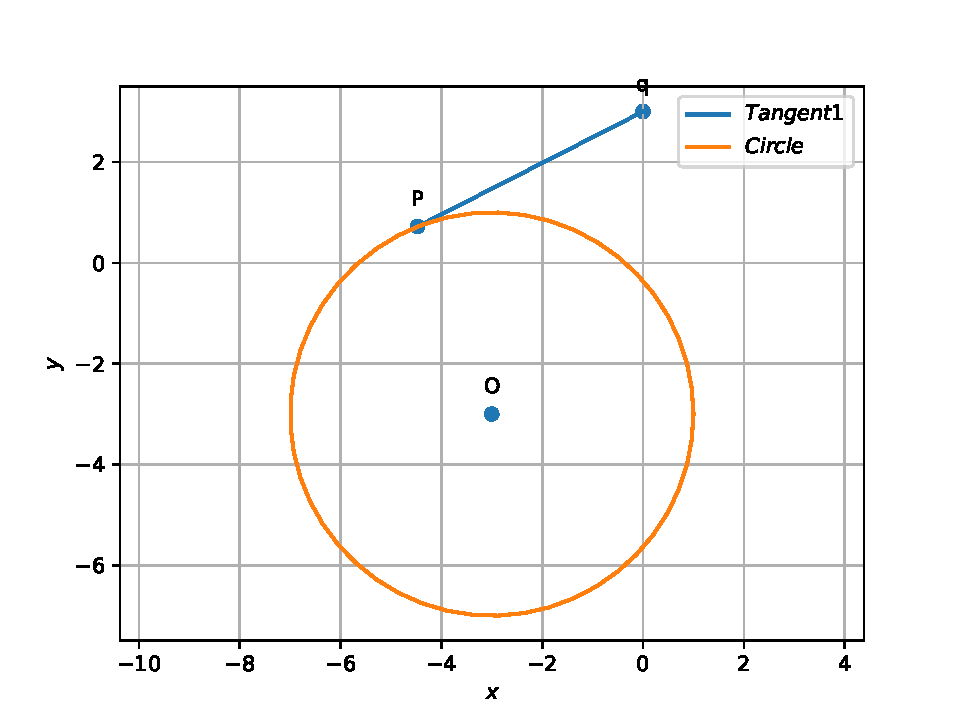
\includegraphics[width=1\columnwidth]{fig}
\caption{}
\end{figure}
\section*{construction}









The line equation is


\begin{align}
5x-2y+6=0
\end{align}

for point Q
\begin{eqnarray}
{(5 \;-2)}
\myvec{x\\y}=-6
\end{eqnarray}


\begin{eqnarray}
\vec{n^Tx}-c
\end{eqnarray}

\begin{eqnarray}
{(5 \;-2)}
\myvec{0\\k}=-6
\end{eqnarray}

\begin{center}
-2k=-6\\
k=3
\end{center}

\begin{eqnarray}
\vec{Q}=\myvec{0\\3}
\end{eqnarray}
Given circle equation is \begin{align}
x^2+y^2+6x+6y-2=0
\end{align}
\begin{align}
\vec{x}^T\vec{Vx}+2\vec{U}^T\vec{x}+f=0
\end{align}
\begin{eqnarray}
V=\myvec{1&0\\ 0 &1} \; u=\myvec{3\\3} \;  f=-2
\end{eqnarray}





let tangent equation

$\vec{x}=\vec{q}+\lambda \vec{m}$\\
where m is found as solution of equation

Where  
\begin{eqnarray}
\vec{\Sigma=(VQ+u)(VQ+u)^T-V(Q^TVQ+2u^TQ+f)}
\end{eqnarray}

 \begin{eqnarray}
	 \vec{p^T\Sigma p}=\vec{D}
 \end{eqnarray}
 






\begin{eqnarray}
\vec{\Sigma}=\myvec{  9 &18\\ 18 &36  } -\myvec{  25 &0\\ 0 &25}
=\myvec{  -16 &18\\ 18 &11  }
\end{eqnarray}
\begin{eqnarray} 
\vec{m^T\Sigma m=0}                       
\end{eqnarray}





length of the tangent
\begin{align}
\vec{\lVert Q +\lambda m-Q\rVert=  |\lambda| \lVert m\rVert}
\end{align}

\begin{center}
$|\lambda|$=$|\frac{-m^T(VQ+u)}{m^TVm}|$\\
$\lambda=1.31$
\end{center}










length of the tangent=5

by using any value of $\mu$










































 
\end{document}
